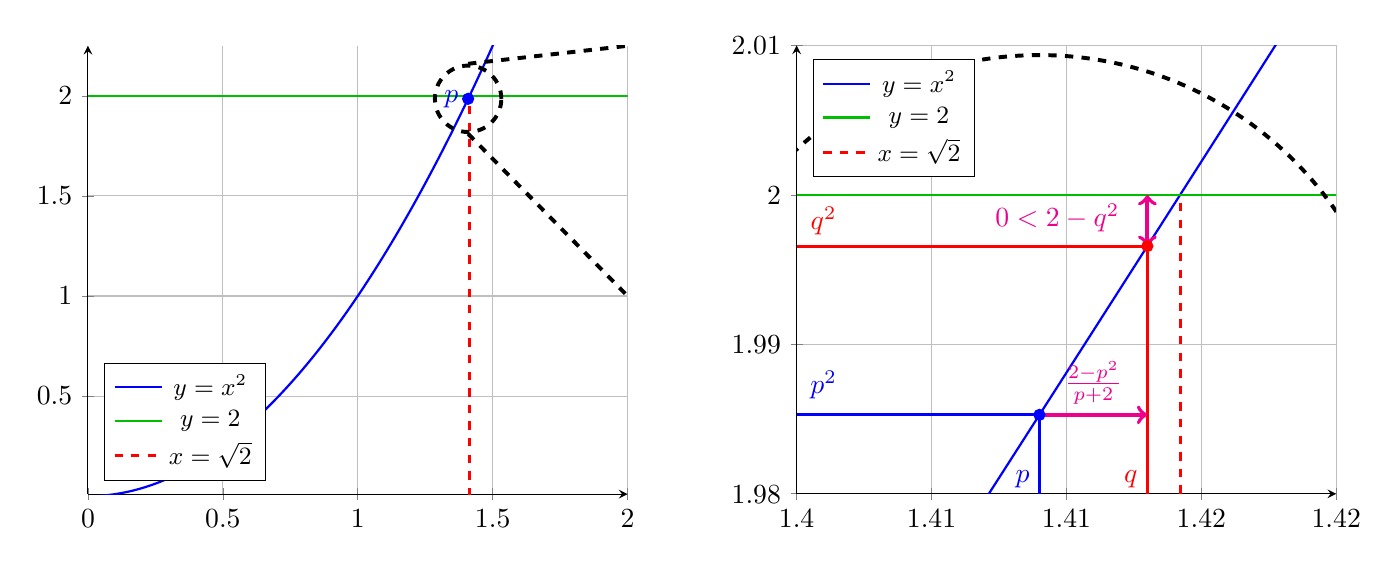
\begin{tikzpicture}[scale=1]
	\begin{scope}[xshift=-9cm]
	\begin{axis}[
		axis lines = left,
		xmin = 0, xmax = 2,
		ymin = 0.01, ymax = 2.25,
		domain=0:2,
		samples=1000,
		grid = both,
		legend pos=south west,
		legend style={font=\small},
		]
		
		% Plot m^2 curve
		\addplot[blue, thick] {x^2};
		\addlegendentry{$y=x^2$}
		
		% Plot line y=2
		\addplot[green!75!black, thick] {2};
		\addlegendentry{$y = 2$}
		
		\addplot[dashed, red, line width=.4mm] coordinates {(1.4142135, 0) (1.4142135, 2)};
		\addlegendentry{$x = \sqrt{2}$}
		
		% Mark an example point m
		\addplot[only marks, mark=*, blue] coordinates {(1.409,1.409^2)};
		\draw[dashed, line width=.5mm] (axis cs:1.409,1.409^2) circle (12pt);
		\draw[dashed, line width=.5mm] (axis cs:1.409,1.409^2-.175) -- (2,1);
		\draw[dashed, line width=.5mm] (axis cs:1.409,1.409^2+.175) -- (2,2.25);
		
%		\addplot[blue, line width=.4mm] coordinates {(1.409,0) (1.409, 1.409^2)} ;
		\node[anchor=east] at (axis cs:1.409,1.409^2) {$\textcolor{blue}{p}$};
%		\addplot[blue, line width=.4mm] coordinates {(1.4,1.409^2) (1.409, 1.409^2)};
%		\node[anchor=north] at (axis cs:1.401,1.9889) {$\textcolor{blue}{p^2}$};
	\end{axis}
	\end{scope}
	\begin{axis}[
		axis lines = left,
		xmin = 1.40, xmax = 1.42,
		ymin = 1.98, ymax = 2.01,
		domain=1.40:1.42,
		samples=1000,
		grid = both,
		legend pos=north west,
		legend style={font=\small},
		]
		
		% Plot m^2 curve
		\addplot[blue, thick] {x^2};
		\addlegendentry{$y=x^2$}
		
		% Plot line y=2
		\addplot[green!75!black, thick] {2};
		\addlegendentry{$y = 2$}
		
		\addplot[dashed, red, line width=.4mm] coordinates {(1.4142135, 0) (1.4142135, 2)};
		\addlegendentry{$x = \sqrt{2}$}
		
		% Mark an example point m
		\addplot[only marks, mark=*, blue] coordinates {(1.409,1.409^2)};
		
		% Mark m' near m
		\addplot[only marks, mark=*, red] coordinates {(1.413,1.413^2)};
		\addplot[red, line width=.4mm] coordinates {(1.413,0) (1.413, 1.413^2)} ;
		\node[anchor=east] at (axis cs:1.413,1.981) {$\textcolor{red}{q}$};
		\addplot[red, line width=.4mm] coordinates {(1.4,1.413^2) (1.413, 1.413^2)};
		\node[anchor=north] at (axis cs:1.401,1.9999) {$\textcolor{red}{q^2}$};
		
		\addplot[<->, line width=.5mm, magenta] coordinates {(1.413,1.413^2) (1.413, 2)};
		\node[anchor=west] at (axis cs:1.407,1.9985) {$\textcolor{magenta}{0<2-q^2}$};
		
		\addplot[blue, line width=.4mm] coordinates {(1.409,0) (1.409, 1.409^2)} ;
		\node[anchor=east] at (axis cs:1.409,1.981) {$\textcolor{blue}{p}$};
		\addplot[blue, line width=.4mm] coordinates {(1.4,1.409^2) (1.409, 1.409^2)};
		\node[anchor=north] at (axis cs:1.401,1.9889) {$\textcolor{blue}{p^2}$};
		
		% Arrow showing the increment
		\draw[->, line width=.5mm, magenta] (axis cs:1.409,1.409^2) -- (axis cs:1.413,1.409^2)
		node[midway, above, sloped] {\(\frac{2-p^2}{p+2}\)};
		
		\draw[dashed, line width=.5mm] (axis cs:1.409,1.409^2) circle (130pt);
	\end{axis}
\end{tikzpicture}